% Chapter 1
\chapter{Problem definition} 
\label{chap_problem_definition}
This chapter presents the context of the thesis, which aims at proposing empirical models to estimate small-scale information of turbulent flows from low resolution measurements. This work is addressed due to the shortage of research tools that could give a complete view of turbulent flows, with information at both large and small scales. The thesis brings forth two problems being solved. The first one is to find functions to estimate high-resolution fields, containing both large and small scales, from low-resolution measurements, essentially large-scale information. The second problem is to find fusion models to combine multiple sources of low-resolution measurements to reconstruct fully resolved velocity fields. The proposed methods will be tested on two direct numerical simulation datasets of either isotropic turbulence or turbulent channel flow at a moderate Reynolds number. The data give access to the full information and permit to conduct various numerical experiments and study the performances of the reconstructions.

\section{Background}
This section briefly reviews the importance of turbulence studies. The main properties of turbulent flows are discussed, notably as a multi-scale phenomenon. The section further emphasizes the importance of studying small scales, which leads to the main motivation of the thesis. 

\subsection{Turbulence}
Turbulence occurs very often in both nature and engineering applications. It appears in our surroundings, since most fluid flows are turbulent. Turbulence scales can be as extremely small as interior of biological cells or as large as flows in geophysics, astrophysics, oceans or atmospheres. In engineering applications, it dominates most flows around vehicles such as cars, ships or airplanes. It also plays key roles in energy production and transformation or inside combustion chambers. A nice review on these applications of turbulence is given by \citet{tennekes1972first, mcdonough2004introductory, george2009lectures}.

Turbulence brings both desirable and undesirable effects. On the one hand, it enhances mixing and transporting matter, momentum and heat. This property is beneficial since it improves fuel-air mixing and accelerates cooling process in combustion chamber for instance. In civil engineering, turbulence helps releasing pollutant streams into the air or ocean more rapidly. It also enhances mass and heat transfer at solid-fluid or fluid-air interface. In aerospace engineering, it helps increasing wall shear stress on aircraft wing and therefore contributes to avoid separation. On the other hand, turbulence also causes serious consequences. Aerodynamics drag is one of the most troublesome problems. Airbus estimates that 10 $ \% $ reduction of drags caused by turbulent boundary layer would result in one billion Euros fuel saving worldwide per year, along with the contribution to reduce pollution. Turbulence is also the main source of aircraft noises. Better knowledge will help to propose strategies of controlling turbulence in beneficial ways and reduce energy footprint in transportation.

Turbulence studies have mainly focused on theoretical aspects after the discovery of Navier-Stokes equations. The experimental researches on fluid flows have only started since O. Reynolds experiment \citep{reynolds1883experimental}, motivating later works on non-dimensional parameters, closure models, and similarity theories for homogeneous and isotropic turbulence. More recent works have mainly focused on large-scale coherent structures and vortex organizations \citep{hutchins2007evidence}. These works are only possible thanks to the rapid progresses in experimental techniques (mostly optical devices using micro and nano technologies) and computing power. These new results help in increasing our knowledge on turbulence nature, hence improving predictive capacity and proposing more accurate turbulence models for commercial software.
	
Despite constant efforts in the last two centuries, turbulence remains very challenging. The problem has been tackled by many great scientists such as Boussinesq, O. Reynolds (19th), Prandtl, Taylor, Kolmogorov (20th), to name only a few. However, it remains one of the last unsolved problems of classical mathematical physics. Analytical solutions are usually not accessible. The most recent works on N-S equations still discuss the existence of the solution \citep{gallagher2003asymptotics, chemin2009wellposedness, gallagher2015some}. The efforts to measure, calculate or model turbulence are also not fully successful in most practical problems due to its properties as a random, multi-scale and three-dimension irregular phenomenon.

\subsection{Importance of small-scale turbulence}

\begin{figure}
\centering
	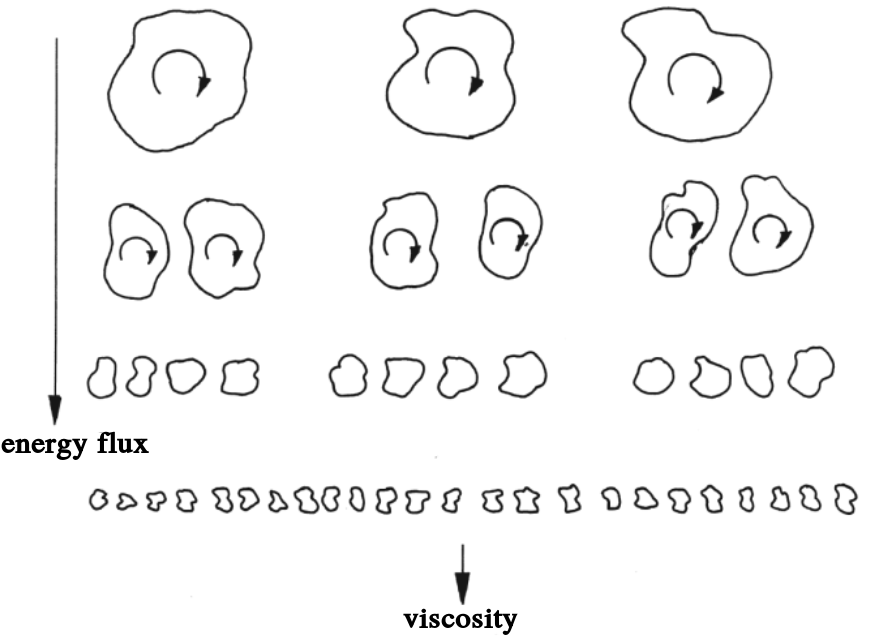
\includegraphics[width=0.75\columnwidth]{./images/probdef/turbulence/energycascade.png}
	\caption{\label{fig:energycascade} Schematic representation of turbulence energy cascade \citep{davidson2015turbulence}, following the sketch by \citet{frisch1995turbulence}.}
\end{figure}

Turbulence is a multi-scale phenomenon, involving scales from the size of the domain till the Kolmogorov dissipative micro-scales. These scales co-exist and interact with each other. Large scales usually contain most of the kinetic energy of the flow, therefore responsible for the transportation of matter, momentum and heat. Small-scale turbulence contains less energy and is strongly involved in the dissipation. Turbulence kinetic energy usually cascades from large to small scales, as schematically represented in figure \ref{fig:energycascade}. The range of scales is continuous, and the width of this range depends on Reynolds number of the flow. 
 
All scales are important to characterize turbulent flows. For instance, an accurate description of all scales is required to estimate full Reynolds stress tensor to validate numerical simulations, turbulence models and scaling theories. This validation is usually performed at very low frequencies, demanding measurements with large field-of-view and long time records. Unsteady flow simulations resolve very small scales in space and time, predict the sharp gradient in the shear layer or near-wall turbulence. Validating these simulations requires small-scale information up to the Kolmogorov length scale.

Small-scale turbulence is crucial to understand the physics of the flow, since they are responsible for the breaking and reconnection of vortices. They are also more likely universal/quasi-universal compared to large scales. A good understanding could lead to turbulence models where the presence of small scales can be parametrized by more universal mathematical models. The efforts to simulate flows could be simplified to large-scale turbulence only, reducing significantly computation costs.  Moreover, small scales are crucial in some contexts such as combustion where matters are brought together at the molecular scales.

\section{Limitations of turbulence research tools}
Despite the constant progress in experiments and numerical simulations, a full access to small-scale turbulence remains impossible for flows at high Reynolds numbers. The section reviews briefly recent advancements and critical limitations. 

\subsection{Numerical simulations}
In academic context, direct numerical simulation (DNS) is the only available tools to directly solve N-S equations without any additional model. It yields all information of the flow via the numerical simulation using an extremely fine grid to resolve all range of scales, from the largest (of the domain size) to the smallest eddies (of the order of the Kolmogorov micro scales). Higher order schemes such as compact finite difference or spectral methods are used to discretize and solve the equations with a very high accuracy.

Constant progress in computational resources permits DNS of higher Reynolds number ($ Re $) and more complex flows. The first attempt of DNS was to simulate isotropic turbulence on a very coarse grid of $ 32^3 $ \citep{fox1972numerical,orszag1972numerical}, while recent simulations of the same flows were performed at $ 4096^3 $ \citep{ishihara2009study,kaneda2003energy}. More complex geometries are also studied, such as channel flows \citep{sillero2013one,lee2014direct}, flat-plate boundary layer under zero and favorable pressure gradients \citep{spalart1986numerical,spalart1988direct} and backward facing step \citep{le1997direct}, among many others.

DNS is limited uniquely to academic context due to computational constraints. The required number of grid points is $ \mathcal{O}\left(Re^{9/4}\right) $ in space and $ \mathcal{O}\left(Re^{3/4}\right) $ in time to resolve the smallest scales. This becomes a real burden for most engineering flows at high $ Re $ and with complex geometries. One of the largest DNS is a channel flow simulation at $ Re_{\tau}\approx 5200 $ \citep{lee2015direct} with the same domain sizes as the well-known simulation by \citet{hoyas2006scaling} at $ Re_{\tau}\approx 2000 $. This is close to $ Re $ of most engineering flows, about $ Re_{\tau}\approx 10^3 $ \citep{smits2013wall}. However, many flows are at $ Re $ one order of magnitude higher and in much more complex geometries. Even when computers become fast enough to simulate those flows, running DNS for engineering flows could produce petabytes of data, which may exceed our capability to analyze and draw useful conclusions.

\subsection{Experimental techniques}
Experiments can provide some information that are not as complete as numerical simulations but for more realistic flows at high $ Re $ and more complex geometries. The most common techniques are hot wire anemometry (HWA) and particle image velocimetry (PIV).

\subsubsection{Hot Wire Anemometry}  
Hot Wire Anemometry (HWA), first proposed by \citet{king1914convection}, is a simple yet accurate technique to measure one-point velocities. The anemometer uses a thin wire at very high temperature submerged into the flow. The flow changes the heat equilibrium around the wire, altering the temperature of the wire. The electronic circuit of the device provide to the wire a controlled amount of electrical current to keep the wire temperature constant. The velocity is deduced from the voltage change. Since the change is analog without any information loss, the temporal frequency of velocity measurements can reach about 100 kHz, which corresponds to Kolmogorov time scale of most realistic flows. The main constraint is the spatial discretization, since only point-wise measurements are possible, and a rake of hot wires soon becomes intrusive.

\subsubsection{Particle Image Velocimetry}  
Particle Image Velocimetry (PIV) is currently the best technique to measure global/topological view of flows. The method aims at recording images of tracers seeded in the flow, which are necessarily light and neutrally buoyant, to measure instantaneous velocity fields \citep{adrian2005twenty,keane1992theory}. Laser light sheets pulsed at a fixed time interval are used to  illuminate a slice of the flow, and pairs of images are recored at the same interval by CCD cameras. Velocity at one point is estimated as the averaged displacement of its neighboring tracers within a so-called ``interrogation window''. The most likely position of a group of tracers inside this window at the next time step is estimated using a correlation technique \citep{sutton1983determination}. Final velocity fields are computed knowing the displacements and the interval between two images of the same pair.

The conventional PIV technique measures two-dimension two-component (2D-2C) velocity fields. \textit{Stereo-PIV (SPIV)} measures two-dimension-three-component (2D-3C) fields \citep{prasad2000stereoscopic}. It uses a system of two synchronized cameras to capture images of a seeded flow. These images are simultaneously taken but with distinct off-axis views so that ``out-of-plane'' velocities can be extracted. These two cameras are usually set up in an angular configuration where the axes of the two cameras are rotated while assuring that they intersect with the object plane along the same axis following the Scheimpflug principle.

\textit{Tomographic PIV} can measure 3D-3C velocity fields. It gives the most complete view of a flow, including the velocity gradient tensor, a crucial measure to validate numerical approaches. Proposed recently by \citet{elsinga2005assessment,elsinga2006tomographic}, the main principles remain analogous to SPIV with important modifications. The illumination of the 3D volume is done with a thicker laser sheet, and 3D velocities are estimated using 3D cross-correlations. Recent measurements can reach 3D-3C fields of a volume of about 200 $ cm^3 $ in water or 50 $ cm^3 $ in air at a frequency of 3 kHz \citep{scarano2013tomographic}. 

\textit{``Shake-The-Box''} (STB) calibration technique aims at improving further the spatial resolution by combining Lagrangian and Eulerian views of a flow. The setup resembles tomographic PIV. The time spacing is required to be of the order of the Kolmogorov time scale to ensure an accurate tracking of particle trajectories. From the time-resolved sequence of tomographic images, STB uses particle image matching to find the Lagrangian trajectory of each particles. Interpolation is used to get velocities on the Euclidean regular grid. This technique ideally reaches the resolution till particle sizes. A recent work using STB permits a resolution of 21 pixels per $ mm^2 $ in a cube of $ 10cm \times 10cm \times 2cm $ at 1 kHZ for a flow at $ Re = 33000$ \citep{schroder2015advances}.

Despite above advancements, PIV is still limited in measuring realistic flows due to optical devices and data processing constraints. The state-of-the-art measurements are still a question of finding compromises among high temporal frequency, high spatial resolution and large field of view. This is due to the following critical limitations. 

The spatial resolution of PIV measurements is limited due to the correlation-based calibration technique. The maximum resolution is constrained by \textit{image density} \citep{keane1992theory}, which is the average number of tracers in an integral window (or interrogation cell). This parameter is very important to determine the measurement quality. Too high image density causes the problem of multiple correlation peaks, while too low image density reduces the possibility to find an image pair for each interrogation window. The optimal choice of image density is about 8-10 tracers per interrogation window, which is a compromise between good spatial resolution and quality of autocorrelation estimate. 

STB can overcome the spatial resolution limits by resolving the fields down to the particle size, but requires a system with a very high sampling frequency. Current PIV systems only reach low frequencies compared to the smallest time scales. State-of-the-art systems can capture up to 10000 frames per second (fps) at a resolution of one mega-pixel \citep{willert2015high}. This fps is very large but still not sufficient for most engineering flows in air. These flows sometimes require measurements at frequencies at least one order of magnitude higher. Moreover, a high speed PIV requires a laser that combines extremely high pulsing frequencies and high power.

\section{Problem definition}
Complete views of turbulent flows at both large and small scales are desired. However, current facilities are not yet available to measure such information. Large-scale  information are gradually available, but small-scale turbulence remains out-of-reach. This work addresses the problem of empirically estimating small-scale information from large-scale measurements. It aims at exploiting available measured data and propose computational methods to reconstruct full fields in new situations. Such methods may permit to go beyond what one can measure, compute or store. The idea of the co-conception approach can be studied, where results from this work potentially paves the way to design experiments or simulations in such way that facilitates the post-processing to recover a maximum level of information.

Though out this thesis, cubic spline interpolation is used to go from low to high resolution. It is used also as the benchmark to compare with the proposed models. Interpolated fields contain no small scales with the frequency higher than the cut-off associated with the grid of measured points, neglecting the aliasing effects due to the subsampling. For this reason, through out this thesis, the term \textit{small-scale} is referred also as \textit{high-frequency} (HF) or \textit{high-resolution} (HR), while \textit{large-scale} has the same meaning as \textit{low-frequency} (LF) or \textit{low-resolution} (LR).

\subsection{Estimating high-resolution turbulent fields from low-resolution measurements}
\label{sec:probdef1}

\begin{figure}
\centering
	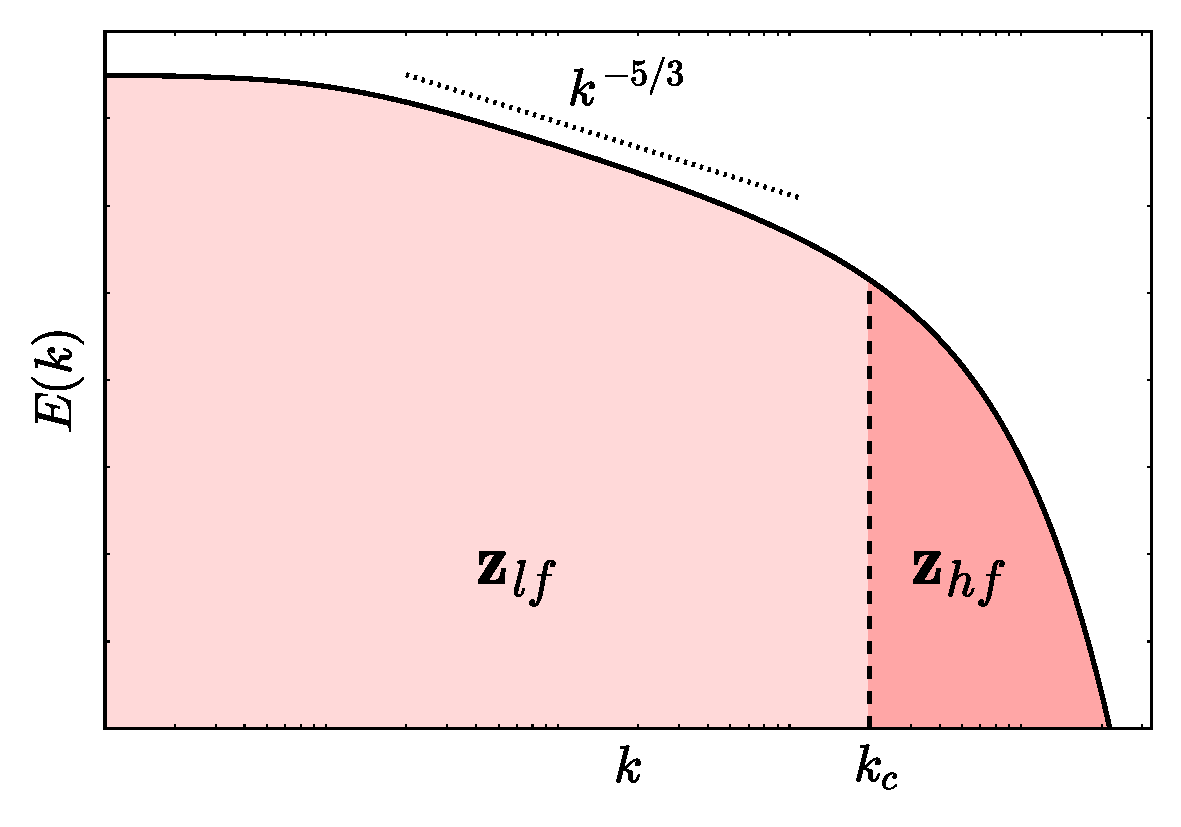
\includegraphics[width=0.6\columnwidth]{./images/probdef/turbulence/turbulence_spectra_long.eps}
	\caption{\label{fig:turbulence_spectra} Turbulence energy spectrum with relative separation between large and small scales by a cutoff wave number $ k_c $.}
\end{figure}

Structures in a turbulent flow can be relatively separated into large and small scales as shown in figure \ref{fig:turbulence_spectra}. Energy content $ E(k) $ is shown as a function of each wave number $ k $ in log-log scale. This Fourier spectrum is continuous, and under certain conditions it has a $ k^{-5/3} $ region. The ranges of scales and their energy contents are very wide depending on $ Re $. Large scales $ \LF $ and small scales $ \HF $ are separated at the cutoff wavenumber $ k_c $. We consider the situation where $ \LF $ - the low spatial resolution or low temporal frequency fields- is measured while $ \HF $ is not accessible. 

The question is \textit{can small scales be estimated from large-scale measurements}? This can be considered as whether a mapping function $ f $ exists such that, given LF measurements, the HF contents $ \HF $ of the flow can be predicted by:
\begin{equation}
f:  \LF \mapsto  \HFest  = f \left(\LF\right)
\end{equation}
No theoretical mapping function exists, although turbulent flows are governed by N-S equations. Despite constant attempts, researchers have not succeeded in proposing turbulence models to represent universal relations between large and small scales.

This thesis aims at proposing empirical functions, either linear and nonlinear, to estimate small-scale information given the large scales. The use of ``empirical'' models is in the sense of learning, where data at all scales are available \textit{a priori}. The proposed algorithms learn from the training data a empirical relation between large and small scales. This relation is presented in the form of a function $ f(.) $, which permits to estimate small-scale information in new situations.

\begin{figure}
\centering
	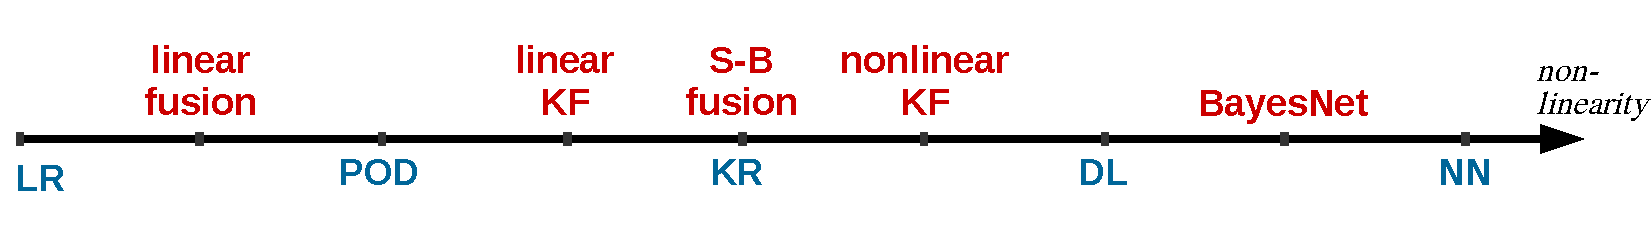
\includegraphics[width=\columnwidth]{./images/probdef/turbulence/models_spectrum.pdf}
	\caption{\label{fig:models_spectrum} Spectrum of models ordered by their level of nonlinearity (from left to right). Methods for mapping large-small scales are in blues, while those for fusion of measurements are in reds. Notations: linear regression (LR), proper orthogonal decomposition (POD), Kalman filter (KF), kernel regression (KR), similarity-based (S-B), dictionary learning (DL), Bayesian network (BayesNet), neural network (NN).}
\end{figure}

A large spectrum of methodologies is discussed and compared. Figure \ref{fig:models_spectrum} lists such methods (in blue) as a function of the order of their nonlinearity. Pure linear models are conventional regression and dimensionality reduction (POD)-based methods. Nonlinearity level grows with model complexity. Simple nonlinear models, the so-called kernel regression, work in a fixed kernel space. The family of dictionary learning methods provides sparse representation of high dimensional data. Neural network, a broader and very active research field, finds nonlinear mapping functions with a more adaptive kernel space. A ``deep'' network permits to model highly nonlinear phenomena. However, we will leave this approach for future works.

\subsection{Fusion of large-scale measurements}
\label{sec:probdef2} 
Turbulence is multi-scale both in space and in time. Usually large or small scales refer to either space (up to three dimensions) or time. However, LF measurements in space potentially contain some HF information in time and vice-versa. One idea is to measure those LF information by different measurement techniques and combine them to infer some HF contents. Such a fusion model takes benefit from each measurement by capturing all possible detailed information. The fused fields contain some small scales that are not accessible from each single measurement. 

\begin{figure}
\centering
	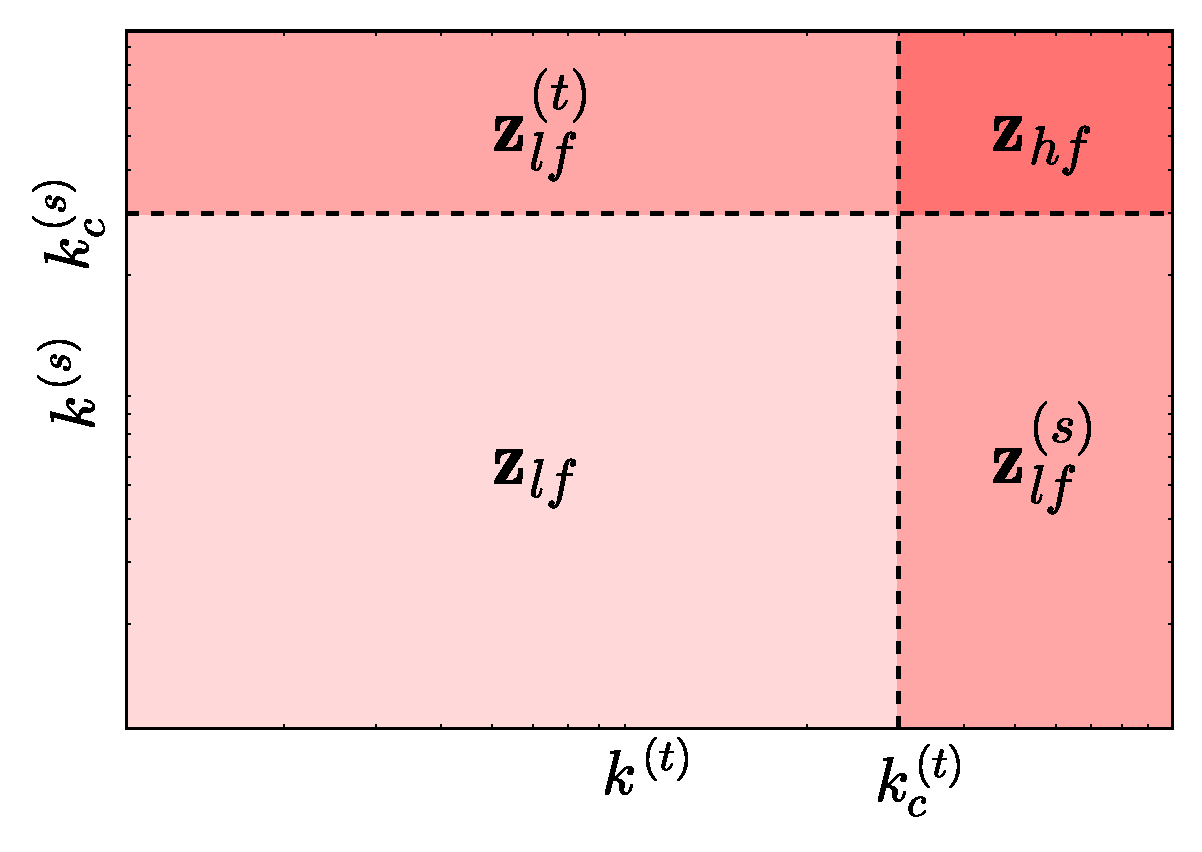
\includegraphics[width=0.5\columnwidth]{./images/probdef/turbulence/space_time_wavedomain_long.eps}
	\caption{\label{fig:space_time_wavedomain} Turbulence energy spectrum with relative separation between large and small scales at wave number $ k_c $.}
\end{figure}

Figure \ref{fig:space_time_wavedomain} depicts schematically the above idea, where LF measurements in space and time are illustrated. In space, two sources of information $ \left\lbrace \LF, \LF^{(s)} \right\rbrace$ are available, where $ \LF $ contains purely LF information in space-time, and $ \LF^{(s)} $ captures LF in space but over the full range of temporal frequencies. An analogous interpretation is for $ \left\lbrace \LF, \LF^{(t)} \right\rbrace $ in time, where $ \LF^{(t)} $ potentially gives some detailed information of the flow in space. By combining two sources of LF measurements in space and time, ideally one can hope to predict all scales in three blocks $ \LF $, $ \LF^{(t)} $ and $ \LF^{(s)} $, while those within $ \HF $ are unreachable. 

\begin{figure}
\centering
	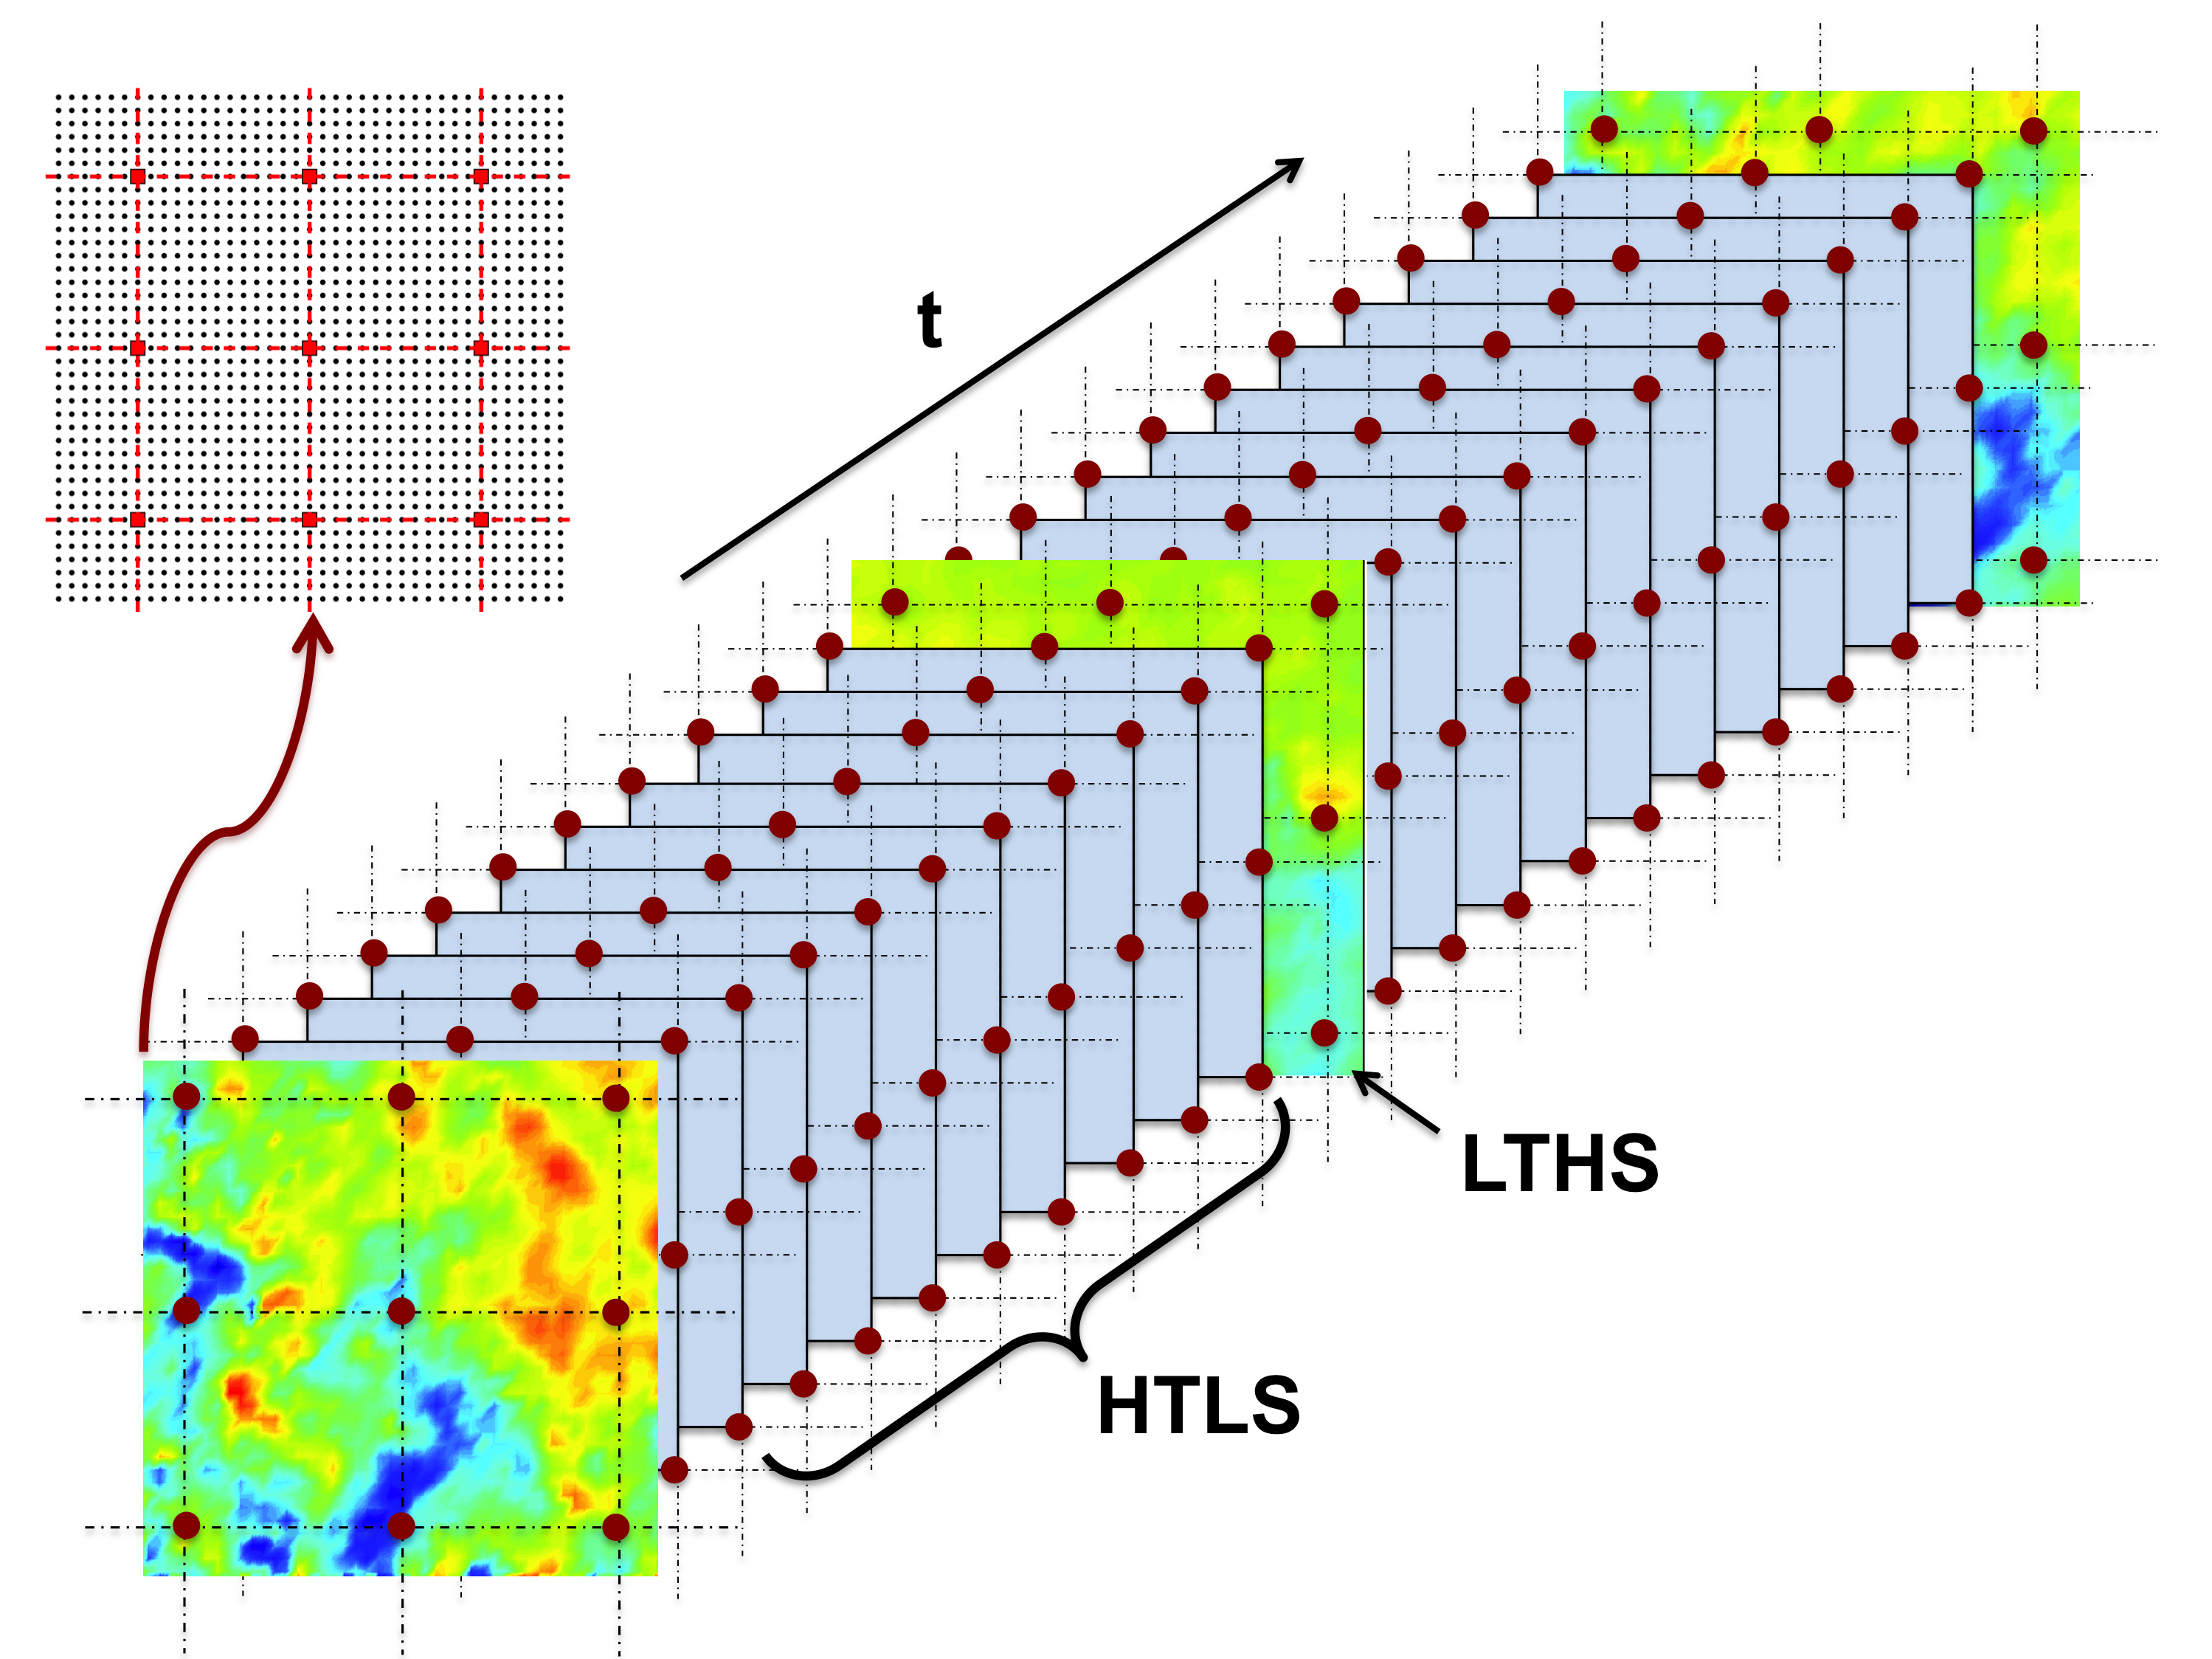
\includegraphics[width=0.5\columnwidth]{./images/probdef/setups/problem_config.png}
	\caption{\label{fig:space-time_measurements} Sketch of the inverse problem, with the two sources of measurements: the LTHS (color images) and a coarse grid of HTLS (red dots among black ones of LTHS). The inverse problem of HTHS data reconstruction is to fill in the space-time data-cube.}
\end{figure}

This work addresses a configuration as in figure \ref{fig:space-time_measurements} where two sources of measurements, the high-temporal-low-spatial (HTLS) and low-temporal-high-spatial (LTHS) resolution velocity fields are available. LTHS measurements (black dots) at the three colorful planes are synchronized with HTLS measured positions at LR (red dots). HTLS captures HF contents of the flow dynamics, while LTHS measures highly resolved information in space. By combining these two sources, one hopes to capture more small-scale information in space and time. 

This idea has been studied at LML in an European joint experiment \citep{coudert2011double}. A database of a boundary layer flow at high $ Re $ was measured using SPIV synchronized with a rake of HWA probes. PIV measurements (LTHS) are with a large field-of-view ($ 30 \times 30 cm $) and a high spatial resolution ($ 143 \times 167 $) but at a low acquisition frequency ($ 4 Hz $). HWA measurements in a rake of probes (HTLS) of the same field-of-view are sampled at an extremely high rate ($ 50 kHz $). However, the spatial discretization is very coarse ($ 11 \times 13 $) compared to the smallest scale. The post-processing step is to estimate velocity fields at the frequency $ 50 kHz$ and the resolution $ 143 \times 167 $.

This work studies computational methods to combine HTLS and LTHS measurements to maximize the information level. The spectrum of possible methods as the order of nonlinearity is shown (in red) in figure \ref{fig:models_spectrum}. For completeness, the idea of data assimilation using linear/nonlinear Kalman filter is mentioned, but further discussion is outside the scope of this work. A fusion approach based on local similarity, the so-called similarity-based (S-B) scales propagation model, is proposed. This method further exploits the local information of the flow, with certain advantages and limitations compared to the linear fusion model. Another fusion method based on Bayesian framework is also proposed, which is further simplified as a linear model.

\section{Datasets}
Experimental data are available from the WALLTURB project \citep{coudert2011double}. However, there is no HR reference data in space-time to qualify and compare different reconstructions. This is the reason why DNS data are used in the present study to access fully resolved velocity fields. Data acquire the true properties of turbulent fields, since DNS simulates flows without any turbulence modeling. The data are also free from measurement uncertainties and noises, making possible a fair comparison of different models. LR measurements are virtually extracted from HR data. The proposed models are learned from these training data to reconstruct fully resolved fields, which are used to estimate the accuracy of different approaches by comparing to reference DNS data.

Two DNS datasets are used . The first data is from the DNS of a turbulent channel flow at a moderate $ Re $. The designed numerical experiments on this data very well imitate the database from LML experiment. However, due to the problem of non-homogeneity, it is challenging for some models to perform. Data of isotropic turbulence is used as well, with further assumptions of isotropy, periodicity and homogeneity, but still retains the principal properties of turbulence.

For both data, the configuration of HTLS and LTHS measurements as in figure \ref{fig:space-time_measurements} is studied, with the following notations to describe. HTHS, HTLS and LTHS snapshots at the $ t-$th time step are denoted as $ \z_t \in \R^{\dimsh} $, $ \y_t \in \R^{\dimsl} $ and $ \x_t \in \R^{\dimsh} $, respectively. The dimension of HR fields ($ \z_t $ and $ \x_t $) is $ \dimsh $, higher than the LR dimension $ \dimsl $ of $ \y_t $. There are $ \dimth $ HTHS and HTLS snapshots, and only $ \dimtl $ LTHS ones ($ \dimtl < \dimth $) sampled at $ t=1,1+1 \times \dimth/\dimtl,1+2 \times \dimth/\dimtl,...,1+(\dimtl-1)\times \dimth/\dimtl $. The matrix form of $ \{\z_t\} $, $ \{\y_t\} $ and $ \{\x_t\} $ are $ \Z $, $ \Y $ and $ \X $ of sizes $ \dimth \times \dimsh $, $ \dimth \times \dimsl $ and $ \dimtl \times \dimsh $ respectively. 

\begin{figure}[t]
\centering
	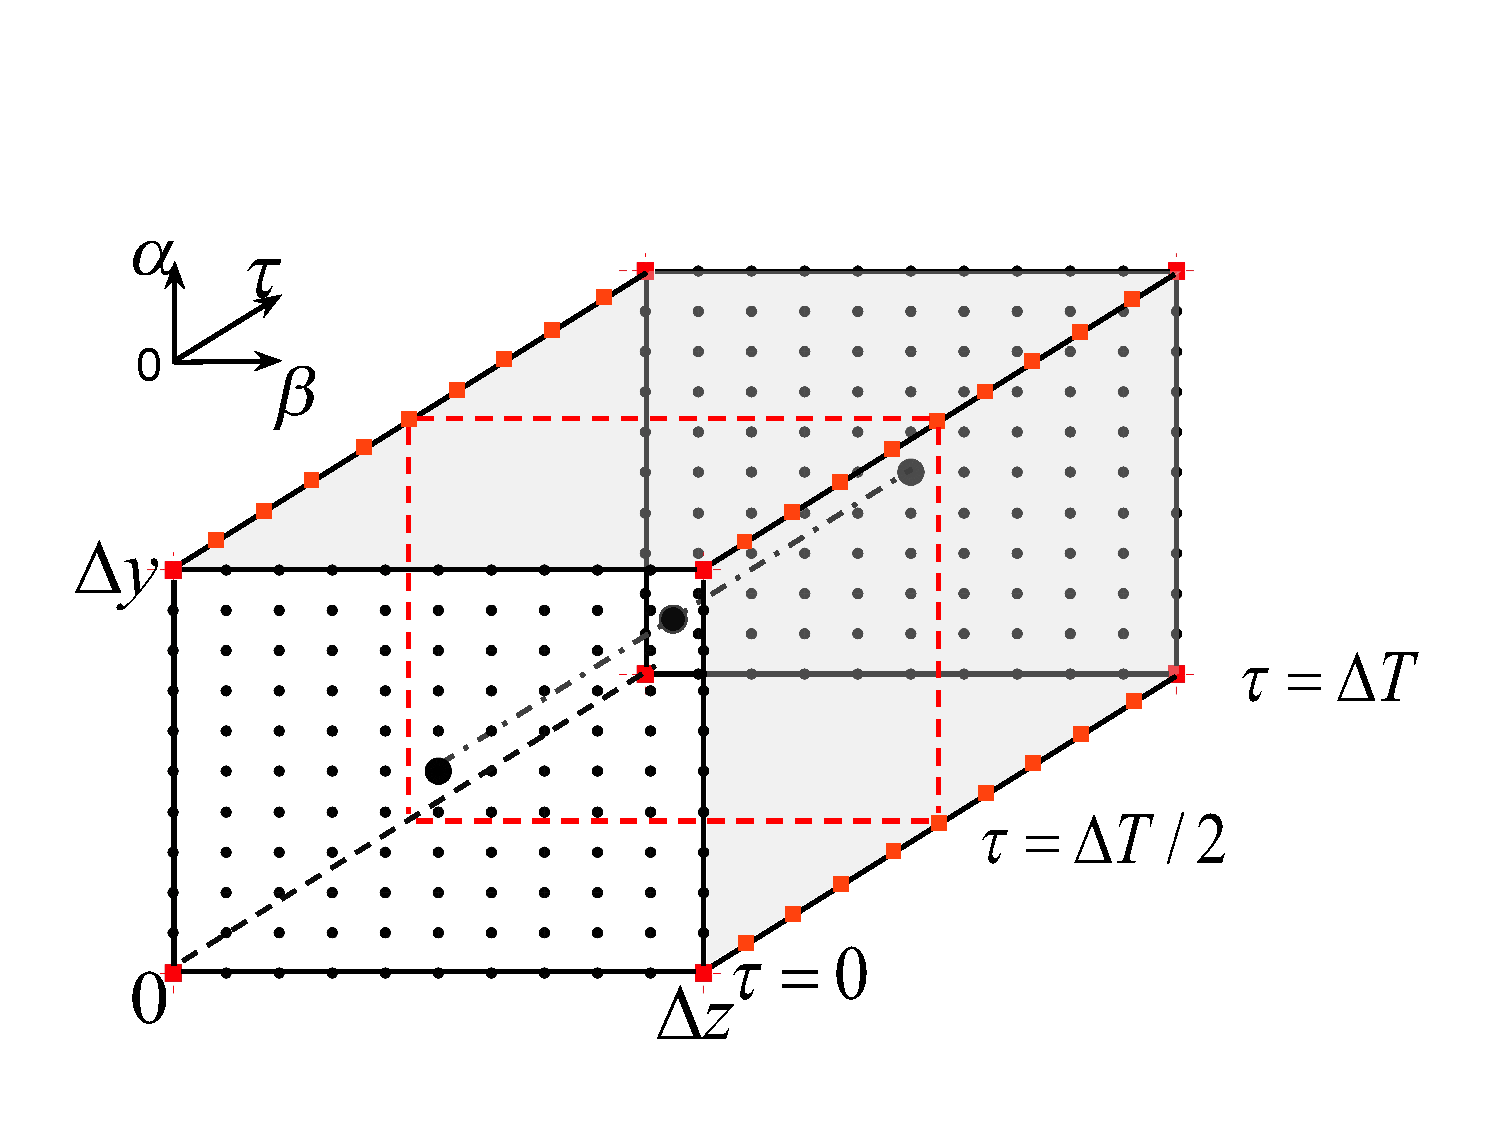
\includegraphics[width=0.6\columnwidth]{./images/probdef/setups/element_block.pdf}
	\caption{\label{fig:element_block} Sketch of an element block with local coordinates $ (\alpha,\beta,\tau) $. LTHS time steps are at $ \tau/\delta t=0 $ and $ \tau/\delta t=\dimth/\dimtl $. HTLS measurements are represented by red dots and LTHS measurements by black ones. }
\end{figure}

To describe all numerical experiments, it is useful also to introduce a sketch of an \textit{element block} bounded by the measurements as in figure \ref{fig:element_block}. This sketch is also used later to characterize performances of all models, since reconstruction accuracies depends on the relative positions in this block. A local coordinate system is introduced. The time position $ \tau $ is defined as a relative distance to two bounded LTHS snapshots (black dots) at $ \tau =0 $ and $ \tau = \Delta T = \dimth\delta t/\dimtl  $ ($ \delta t $ is the time distance between two neighboring HTLS planes). In space, each plane at $ \tau $ is bounded by the four HTLS measurements at the four corners (red points). The distances between two neighbors are $ \Delta y  = \delta y\sqrt{\dimsh/\dimsl} $ in vertical and $ \Delta z = \delta z\sqrt{\dimsh/\dimsl} $ in spanwise direction. $ \delta y $ and $ \delta z $ are spatial grid sizes in vertical and spanwise direction respectively. We assumed also the sampling ratio are equally $ \sqrt{\dimsh/\dimsl} $ in both directions. The most difficult positions to estimate are at local coordinate $ (\alpha, \beta, \tau) = (\Delta y/2,\Delta z/2,\Delta T/2)  $.

The following parts describe the two datasets in detail.

\subsection{DNS data of channel flow}
\label{sec:data_channel} 
\begin{table}
	\caption{\label{tab:energyloss_chanel}
	Configuration parameters of three subsampling cases in space and three in time for DNS channel flow data. The subsampling ratios of HTLS measurements are $ \sqrt{\dimsh /\dimsl } $ and equal in both spatial directions. The ratios of LTHS measurements in time are $ \dimth/\dimtl $. The equivalent spacing in spanwise direction is normalized by half channel height as $ \Delta z/H $ and the spacing in time is $\Delta t$. The normalized energy losses in space $\Delta\kappa_s$ and in time $\Delta\kappa_t$ are defined in equation \ref{eq:RMS_losses}.}
	\vspace{.5cm}
	\centering
	\begin{tabular}{lcS[table-format=1.2]S[table-format=1.2]S[table-format=1.2]cS[table-format=1.2]S[table-format=1.2]S[table-format=1.2]} 
		\toprule
		& & \multicolumn{3}{c}{Space} & & \multicolumn{3}{c}{Time} \\
		\cmidrule{1-1} \cmidrule{3-5} \cmidrule{7-9} 
		Subsampling ratio &  & 5  & 10 & 20 & & 4 & 10 & 20\\ %\addlinespace
		Spacing &  & 0.05  & 0.11 & 0.22 & &  0.10 & 0.25 & 0.50\\ %\addlinespace
		\myrowcolour
		Energy loss $\Delta\kappa$ $ (\%) $ &  & 1.23  & 7.08 & 20.83 & & 01.88 & 9.02 & 24.31 \\ %\addlinespace
		\bottomrule
	\end{tabular}
\end{table}

\begin{figure}[t]
	\centering
	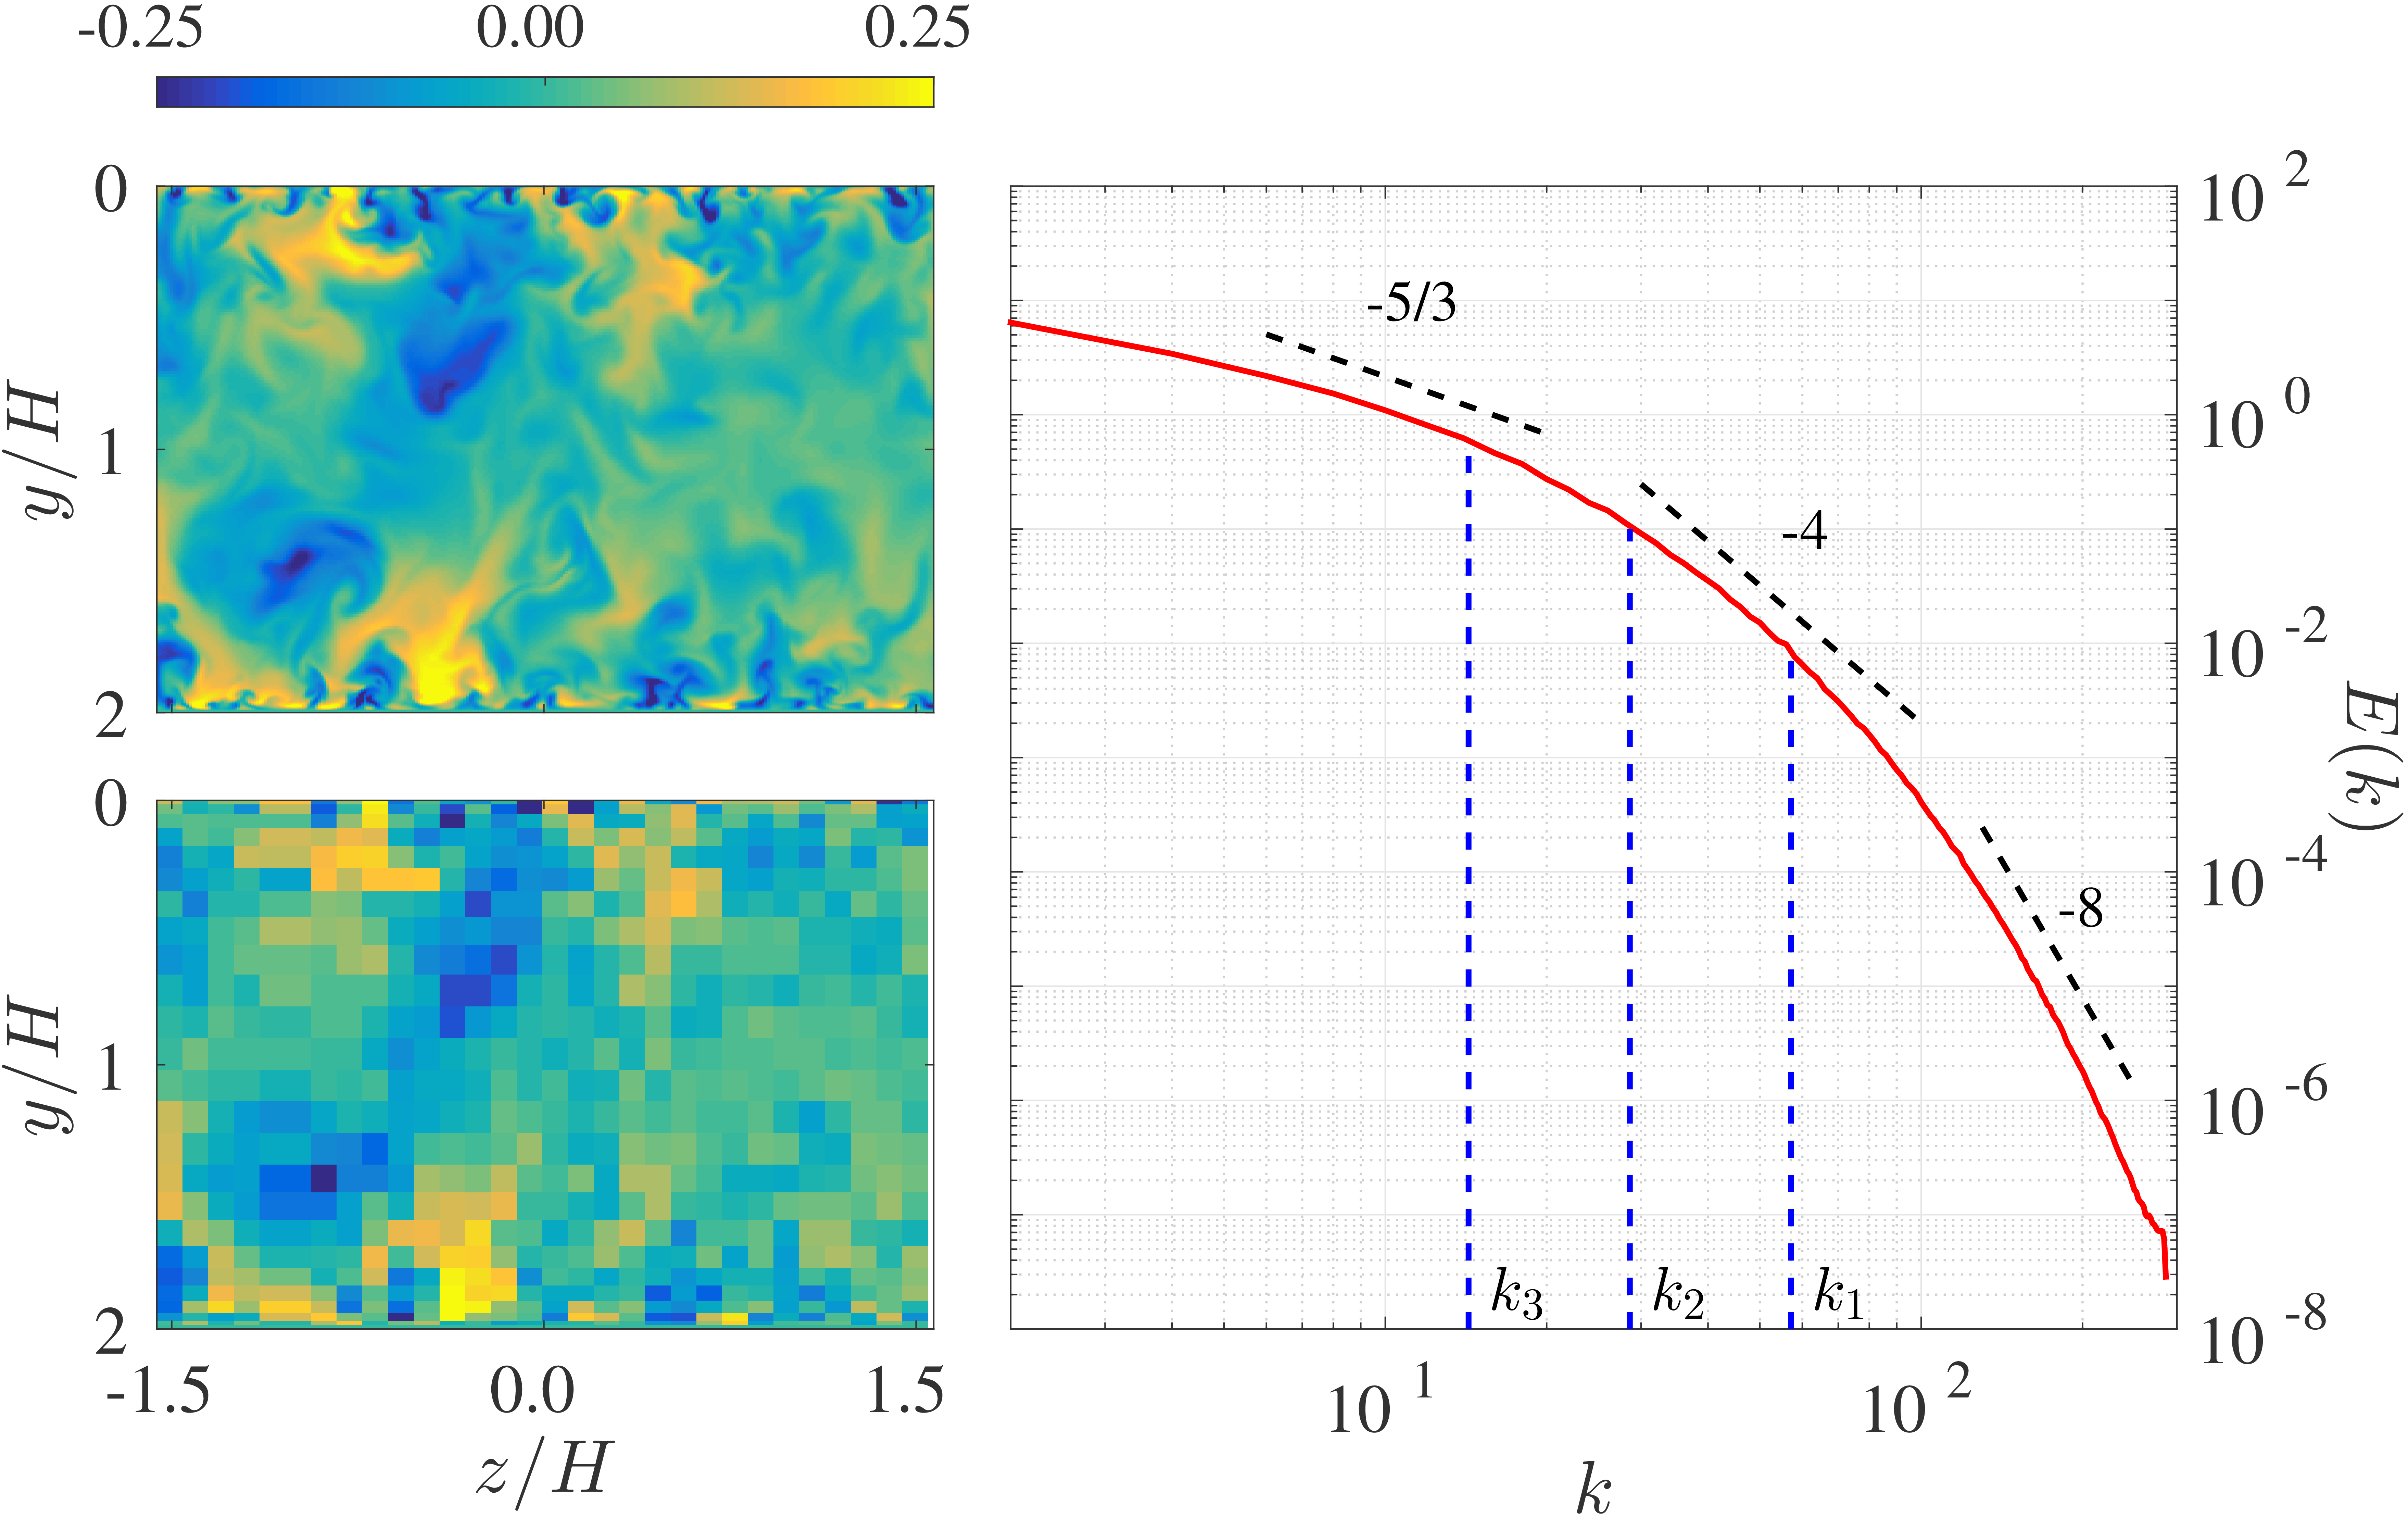
\includegraphics[width=\columnwidth]{./images/datstats/channel/samplevels_spectrum_spanwise_refDNS.png}
	\caption{\label{fig:channel_samplesnap_2D} A sample 2D streamwise velocity of simulated channel and its subsampled field by a factor of 10 (left). This subsampling ratio corresponds to the cut-off wave number $ k_2 $in the plot of spectrum (right) for horizontal lines at the center of the channel. Other wave number $ k_1 $ and $ k_3 $ correspond to the subsampling ratio in space of $ 5 $ and $ 10 $ respectively. }
\end{figure}

DNS database of a turbulent wall-bounded flow is designed the same way as experimental ones. The simulation uses the numerical procedure described in \cite{marquillie2008direct}.
The flow is at a Reynolds number $ Re_{\tau}=550 $ based on the friction velocity $ u_{\tau} $. Cartesian coordinates of the simulation in space are $ (x,y,z) $ for streamwise, vertical and spanwise directions respectively. The domain size normalized by half the channel height $ H $ is $ 2\pi \times 2 \times \pi $. Fully resolved fluctuating streamwise velocities in a plane normal to the flow direction are considered as HTHS data. This data includes $ \dimth=10000 $ snapshots over a grid of $ \dimsh = 288 \times 257 $ points and at a sampling frequency of $ f=\frac{H}{\delta t U_{max}} = 40 $, subsampled from the original simulation at $ f = 200  $. $ U_{max} $ is the central velocity of the flow. LTHS and HTLS measurements subsampled from HTHS data are used to train different prediction models. HTHS is used as the ground truth to estimate reconstruction errors. The extension to spanwise and vertical velocity components follows the same procedure.

Various subsampling ratios both in space and time are considered. In space, the LR fields are obtained by applying a direct subsampling ratio of $ \sqrt{\dimsh /\dimsl } = 5, 10 $ or $ 20 $ in both spatial directions. These ratios correspond to a number $ \dimsl  $ of virtual HTLS sensors of $ 51 \times 57 $, $ 26 \times 29 $ and $ 13 \times 15 $ respectively. Each ratio has a spacing between two successive HTLS points in spanwise and vertical directions of $ \Delta z $ and $ \Delta y $. To test the idea of combining space-time sparse measurements, these subsamplings in space are used together with subsamplings in time of ratios $ \Delta T = \dimth/\dimtl = 4, 10$ or $ 20 $, corresponding to the total number of snapshots $ \dimtl  = 2500, 1000 $ and $500 $ respectively. Each ratio, both in space and time, corresponds to a certain amount of kinetic energy loss. This is essentially the energy of small scales separated from the large ones by a low pass filter (LPF) $ \LPF $. In practice $ \LPF $ will be the $ 5^{th}-$order least square spline filter, either 1D in time ($ \LPF_t $) or 2D in space ($ \LPF_s $), using measurements as knots. This spline filter has the advantage of a sharp cutoff response with a finite support. The energy loss is defined by comparing the filtered field $ \LPF\z  $ to the original field $ \z  $: 
\begin{equation}
	\Delta\kappa=\frac{\displaystyle \sum\limits_{j\in \varmathbb{J}} \z _j^2-\sum\limits_{j\in \varmathbb{J}}{[\LPF\z ]_j^2}}{\displaystyle \sum\limits_{j\in \varmathbb{J}}\z _j^2}
	\label{eq:RMS_losses}
\end{equation} 
where $ \varmathbb{J}$ is the considered set of points. Table~\ref{tab:energyloss_chanel} gathers the energy loss in time ($ \Delta\kappa_t $) and in space ($ \Delta\kappa_s $) estimated with $ \LPF_t $ and $ \LPF_s $ respectively. The set $ \varmathbb{J}$ here contains all points at the center line of the channel, i.e. $ y/H=1 $.

\subsection{DNS data of isotropic turbulence}
\label{sec:data_isotropic}
\begin{figure}[t]
	\centering
	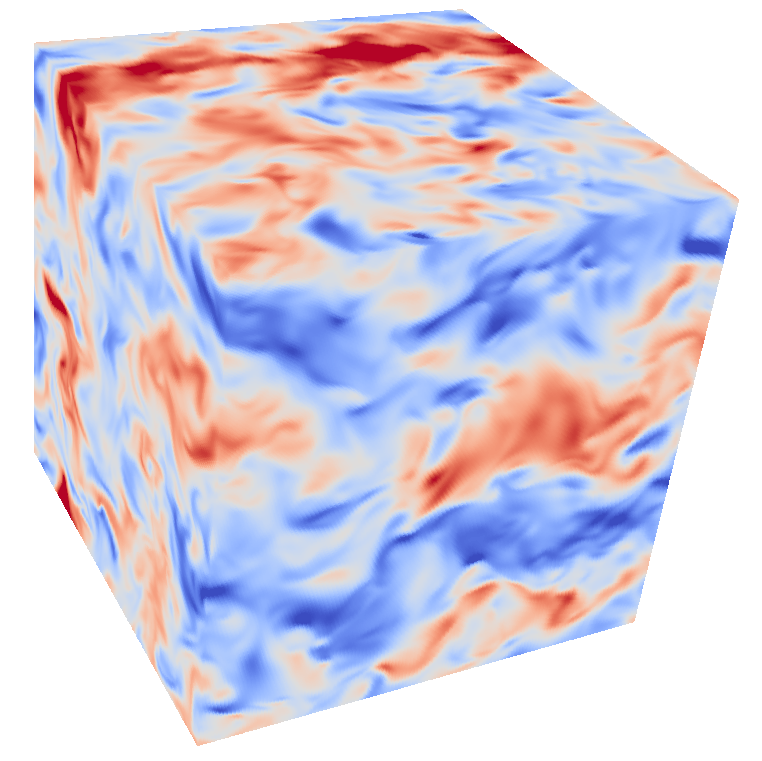
\includegraphics[width=0.45\columnwidth]{./images/datstats/isotropic/velocity_x_3D.png}
	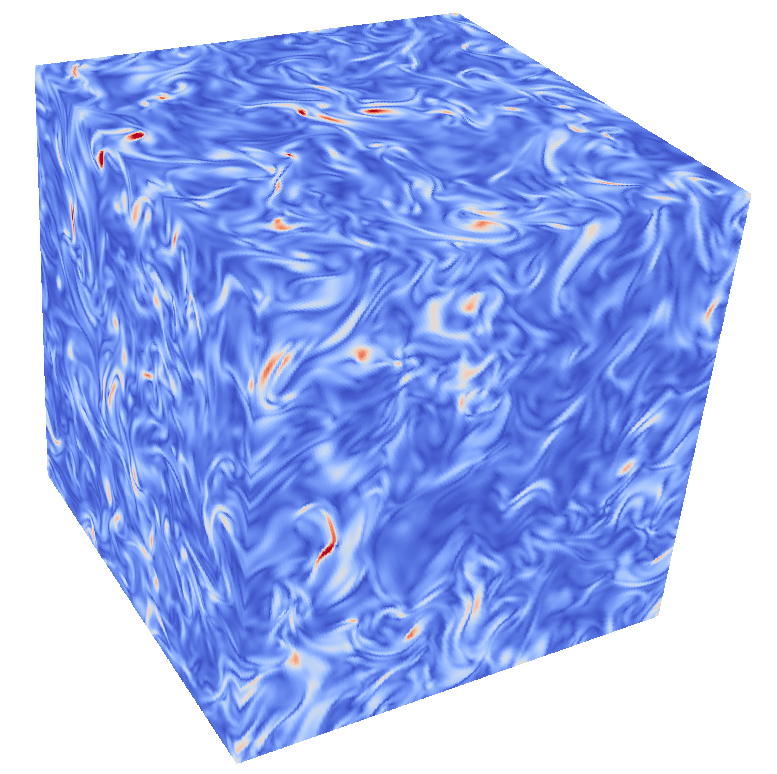
\includegraphics[width=0.45\columnwidth]{./images/datstats/isotropic/vortices3D.png}
	\caption{\label{fig:vortices3D} A sample 3D streamwise velocities (left) and vortices magnitude (right) of DNS isotropic turbulence at $ 384^2 $. The streamwise direction is considered as ``time'' dimension in this case. }
\end{figure}

Channel flows with strong nonhomogeneity in vertical direction yields varying statistics in this direction. Numerical tests of different methods and comparisons of results are more challenging. This nonhomogeneity also calls for a very large database, since all the averaging can be done only in spanwise direction (roughly at the center of the channel) and time. The DNS database of \textit{homogeneous isotropic turbulence} is used for simplifications yet retaining essential properties such as three-dimensionality, intermittency and multi-scale vortices. This flow is assumed to be incompressible inside a periodic box with nearly homogeneous and isotropic statistics. The data are recorded from a simulation over a $ 384^3 $ grid using the Fourier spectral method as originally proposed by \citet{orszag1972numerical}. Figure \ref{fig:vortices3D} shows a sample of a 3D streamwise velocity and vorticity magnitude. $ Re $ is relatively low compared to the state-of-the-art  $ 4096^3 $ simulations by \citep{kaneda2003energy,ishihara2009study}. However, for the purpose of this work, the position of the cut-off frequency is the key parameter and the width of the inertial range is not crucial. Reconstruction accuracy is expected to depend more on the energy loss due to subsampling rather than on $ Re $. Also, the accuracy depends on the slope of the energy spectra at the cut-off frequency, which represents the physics of the flow and implies the level of correlation between neighboring scales

A total of 37 blocks of 3D fields at resolution $ 384^3 $ is recorded. Since a long record of time-resolved data is not available, the streamwise direction is virtually considered as the ``time'' dimension to homogenize the notations for the two datasets. These data are then downsampled by a factor of 4 in every dimension using an ideal Fourier filter, resulting in 3D fields on a $ 96^3 $ grid. The objective is to avoid working within the dissipative range where energy content is very low, leading to a too small energy loss for a given subsampling ratio. Also, the slope of the spectrum is rather high, implying very weak level of correlation between the measured scales and the ones to be reconstructed. Only a small subsampling ratio will now lead to a significant loss, therefore avoiding to work with large ratios and corresponding large numbers of uncertainty. The cubes of $ 96^3 $ are now considered as the reference HTHS fields. Only streamwise velocities in a plane normal to the flow direction are extracted. LR fields will be obtained by virtually subsampling from reference HR ones. A completely analogous procedure is applied to other velocity components.

\begin{figure}[t]
	\centering
	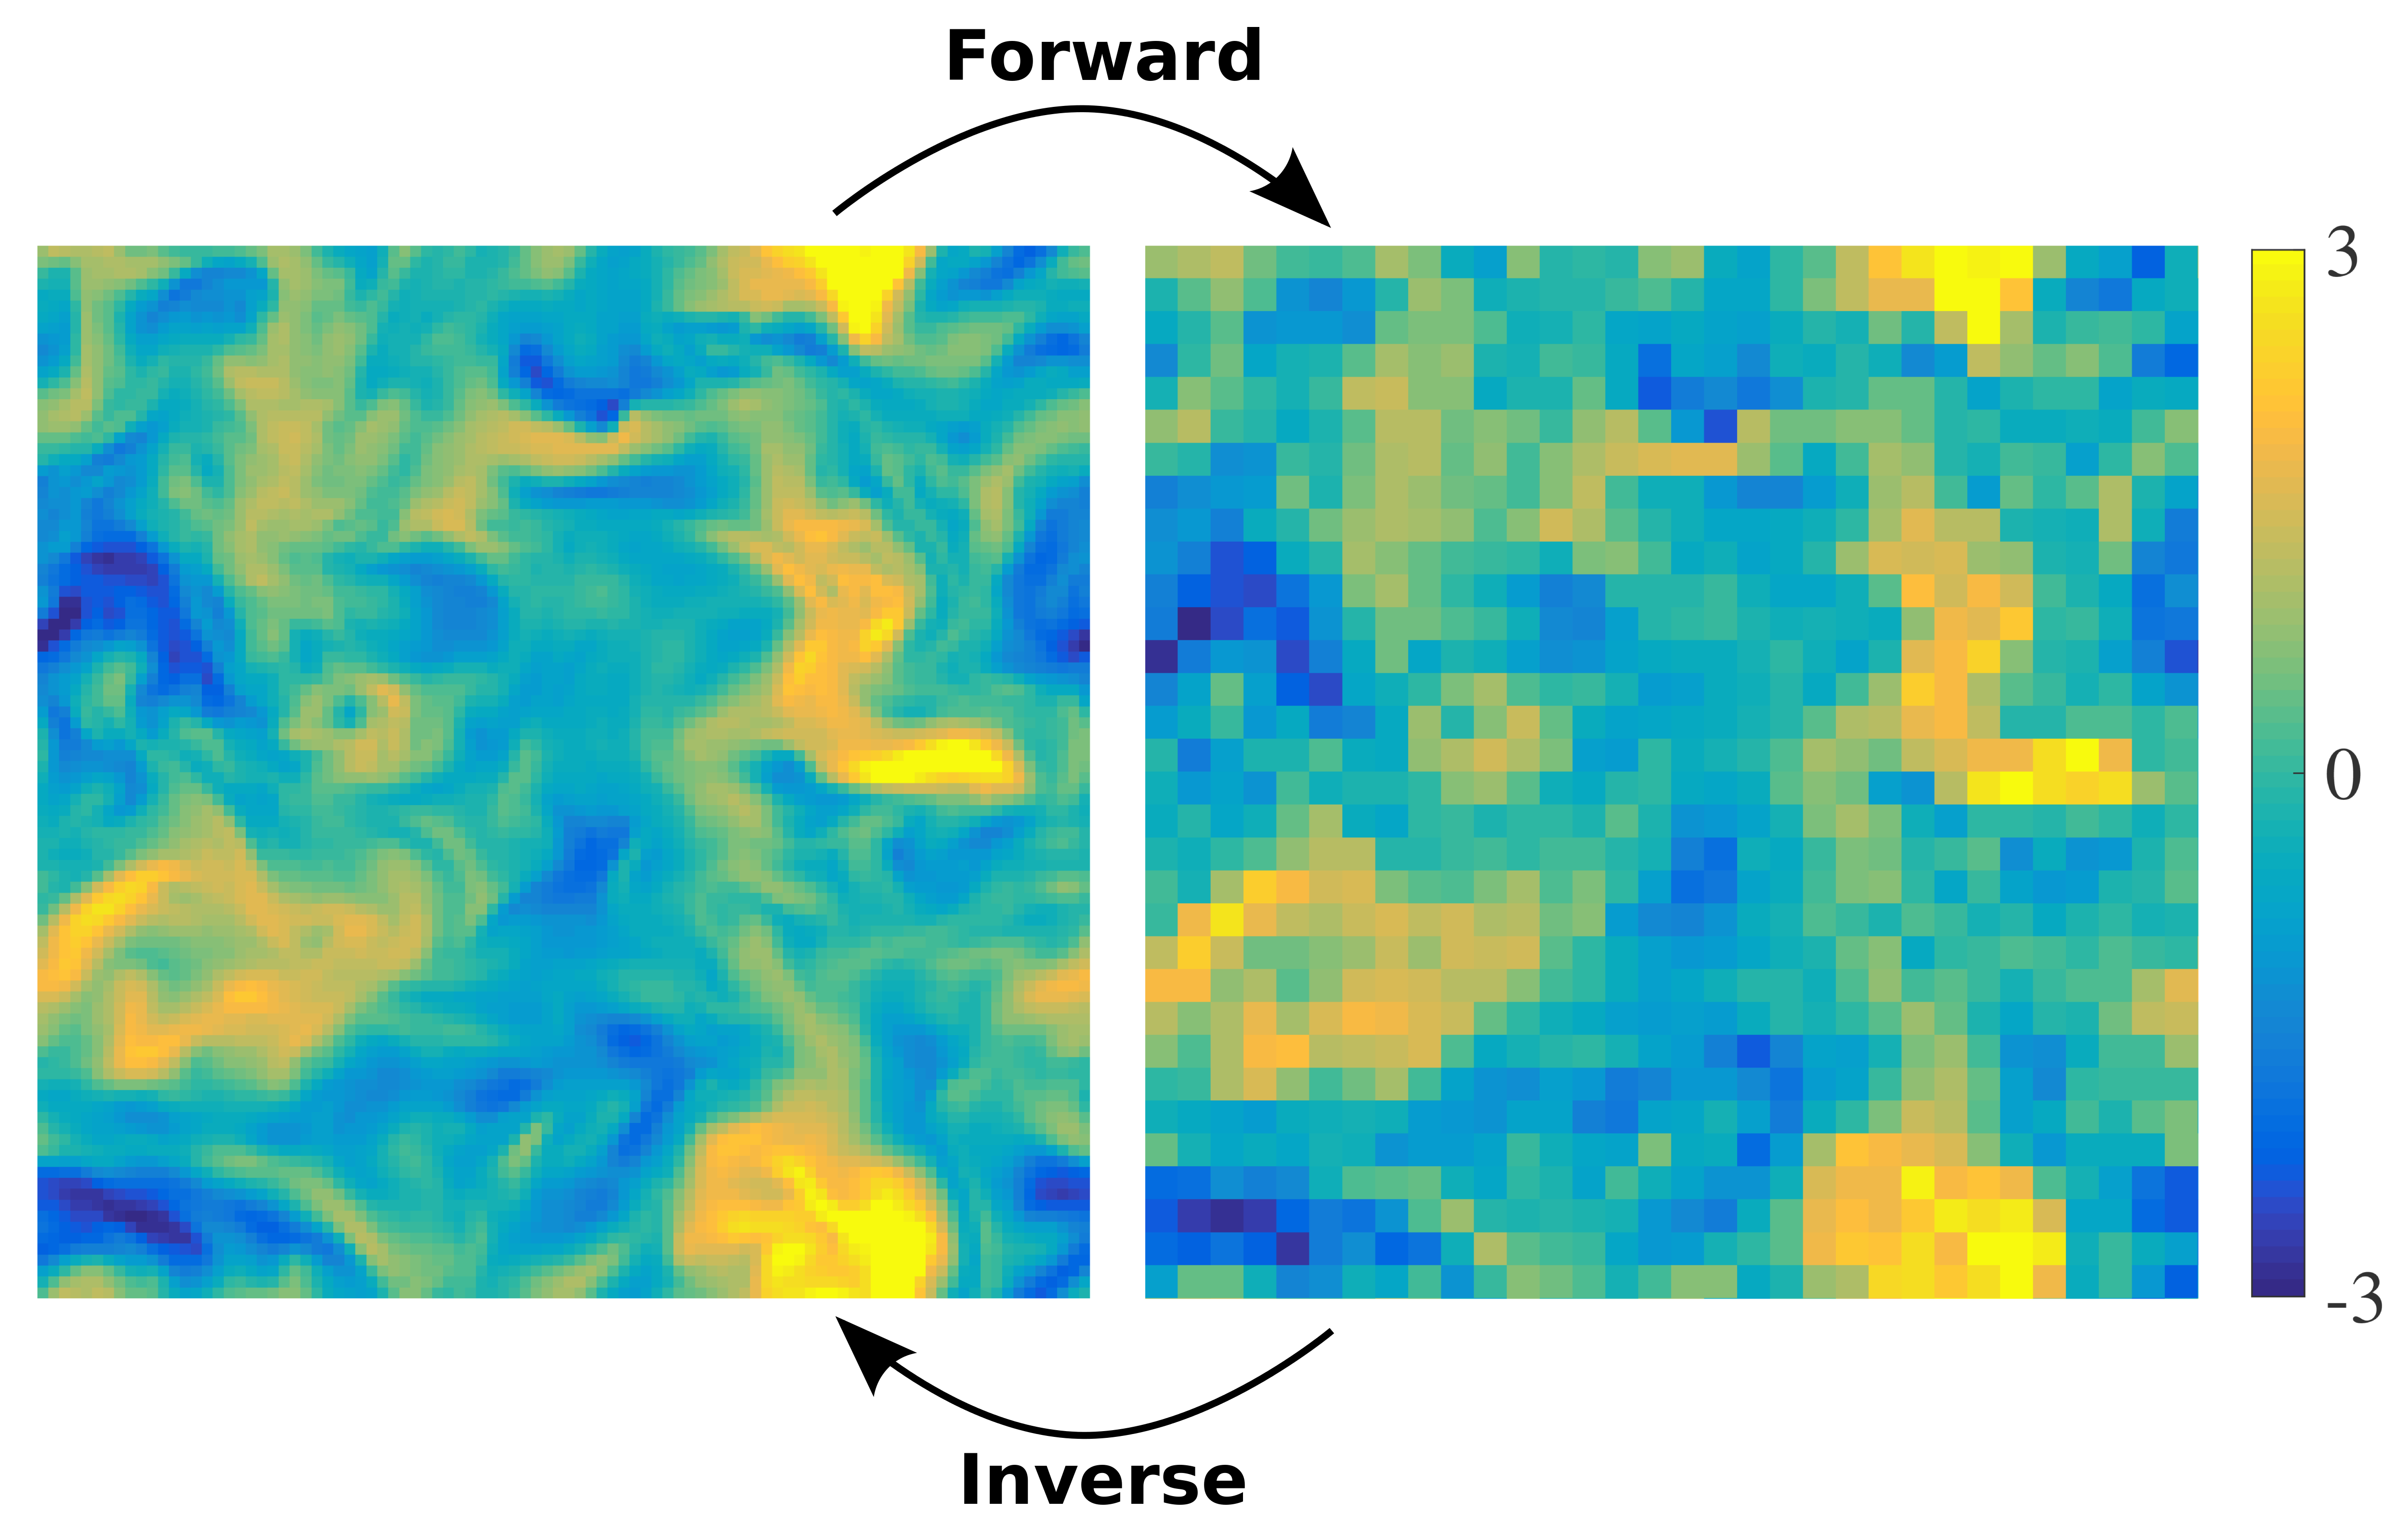
\includegraphics[width=0.8\columnwidth]{./images/datstats/isotropic/u_HR_2D_2.png}
	\caption{\label{fig:u_HR_2D} A sample isotropic 2D streamwise velocity (left) and its subsampled field by a factor of 3 (right) on the plane normal to flow direction. The subsampling is a forward problem, while going from a subsampled to fully-resolved field is an inverse problem.}
\end{figure}

\begin{table}
	\caption{\label{tab:energyloss_isotropic}
		Configuration parameters of three subsampling cases in space (spanwise+vertical direction) and three in time (streamwise direction) for isotropic turbulence data. The subsampling ratios of HTLS measurements are $ \sqrt{\dimsh /\dimsl } $ and equal in both spatial directions. The ratios of LTHS measurements in time (spanwise in this case) are $ \dimth/\dimtl $. The normalized energy losses in space $\Delta\kappa_s$ and in time $\Delta\kappa_t$ are defined in equation \ref{eq:RMS_losses}. The slopes are purely to qualify the steepness of the spectrum and have no physical meaning.}
	\vspace{.5cm}
	\centering
	\begin{tabular}{lcS[table-format=1.2]S[table-format=1.2]S[table-format=1.2]cS[table-format=1.2]S[table-format=1.2]S[table-format=1.2]} 
		\toprule
		& & \multicolumn{3}{c}{Space} & & \multicolumn{3}{c}{Time} \\
		\cmidrule{1-1} \cmidrule{3-5} \cmidrule{7-9} 
		Subsampling ratio &  & 3  & 4 & 6 & & 4 & 6 & 8\\ %\addlinespace
		\myrowcolour
		Energy loss $\Delta\kappa$ $ (\%) $ &  & 1.03  & 2.63 & 7.29 & & 1.23 & 3.56 & 6.53 \\ %\addlinespace
		\bottomrule
	\end{tabular}
\end{table}

\begin{figure}[t]
	\centering
	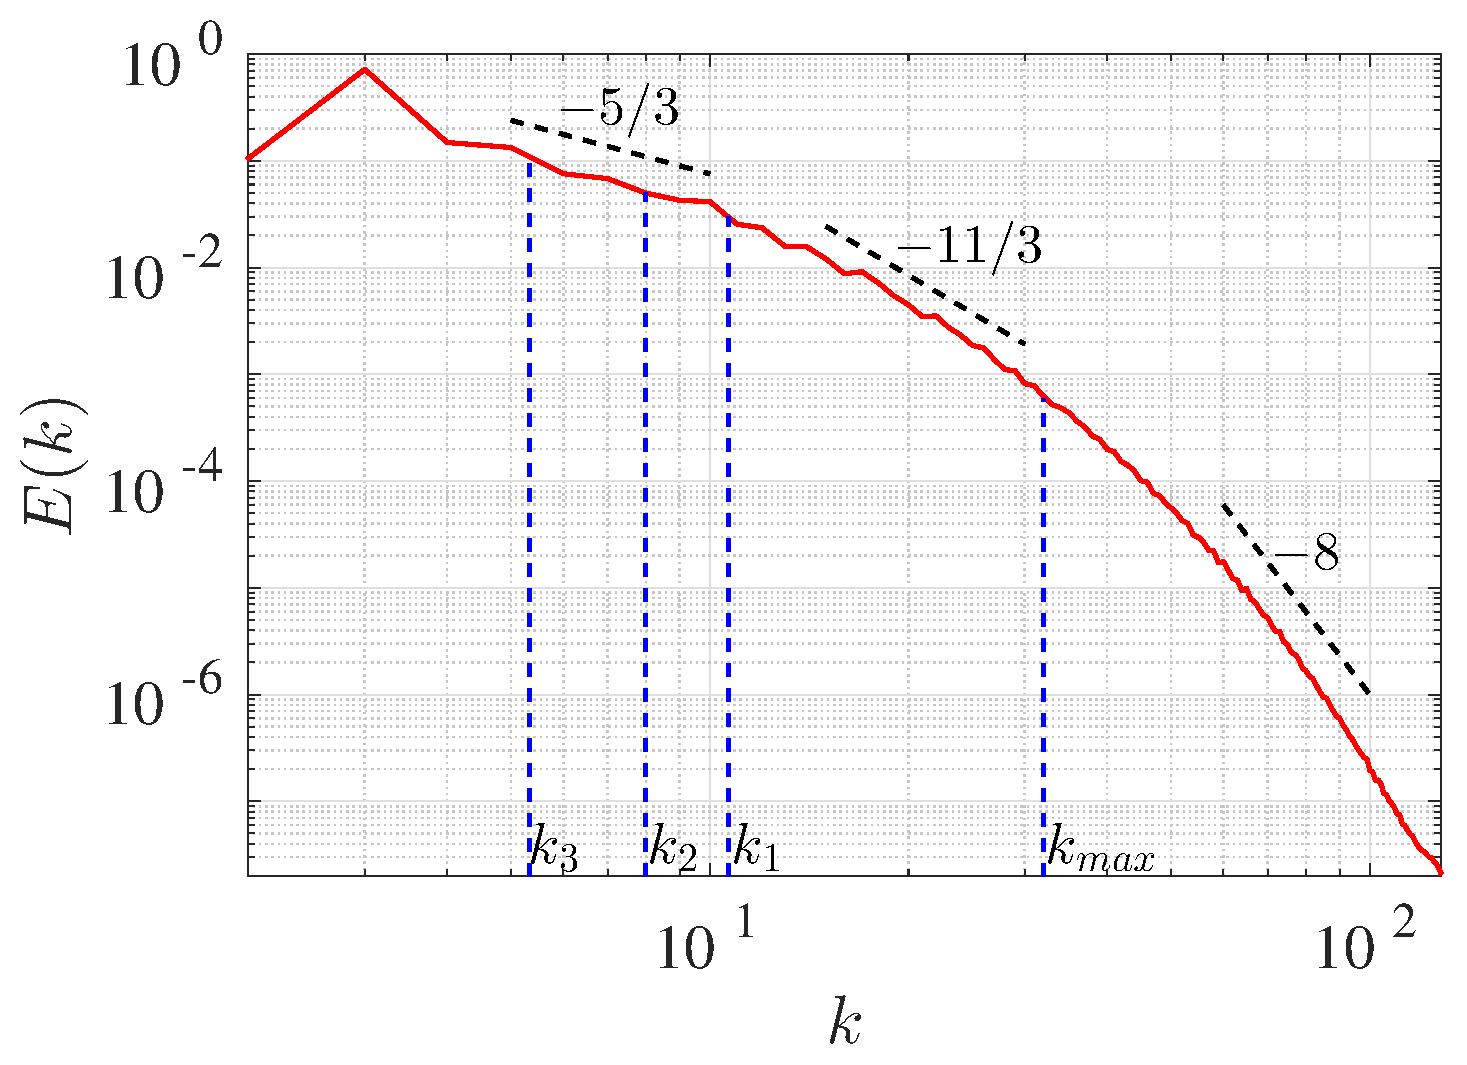
\includegraphics[width=0.65\columnwidth]{./images/datstats/isotropic/spectrum2d_DNS.eps}
	\caption{\label{fig:spectrum2d_DNS} 2D energy spectral of the reference DNS of resolution $ 396^3 $. The maximum real wave number is $ k=128 $ after removing the aliasing contents. Different cutoff wave numbers are shown: $ k_{max} =128/4$ corresponding to the pre-downsampling,  $ k_1 = k_{max}/3 $,  $ k_2 = k_{max}/4 $ and ,  $ k_3 = k_{max}/6 $ for subsampling ratios of $ \sqrt{\dimsh /\dimsl }=3,4 $ and $ 6 $ respectively.}
\end{figure}

Various cases with different ratios are investigated. The subsampling ratios $ \sqrt{\dimsh /\dimsl } $ applied in each direction of space are 3, 4 and 6. These ratios correspond to a number $ \dimsl  $ of HTLS sensors  of $ 32 \times 32 $, $ 24 \times 24 $ and $ 16 \times 16 $ respectively. A sampled HR field with its corresponding subsampled LR field of ratio $ 3 \times 3 $ is shown in figure \ref{fig:u_HR_2D}. Subsampling ratios $ \dimth/\dimtl $ in spanwise direction are 4 , 6 and 8, corresponding to the number of training planes (or key frames) of $ \dimtl =24 $, $ \dimtl =18 $ and $ \dimtl =12 $. Each ratio corresponds to a certain amount of energy loss due to small scales filtered out by an ideal Fourier filter. The energy loss is defined by comparing the filtered fields to the reference ones as in equation \ref{eq:RMS_losses}. The set $ \varmathbb{J}$ now consists of all points thanks to isotropy and homogeneity properties. Table~\ref{tab:energyloss_isotropic} gathers the energy loss due to the 2D or 1D subsamplings.

\section{Concluding remarks}
This chapter has briefly presented the context of the thesis, with the shortage of research tools to measure and compute small scales of turbulence. This problem call for computational methods that permit to estimate such scales from available measurements. We will tackle this problem by seeking: (i) empirical mapping functions between large and small scales, and (ii) fusion models to combine complementary measurements. A wide spectrum of methodologies will be discussed, and their performances will be analyzed using two DNS datasets of either channel flow or isotropic turbulence. Both sets give access to fully resolved fields and permit to design different numerical experiments of various subsampling ratios to obtain virtual measurements. Each configuration is characterized via the kinetic energy loss due to the subsampling. 